% Asset ID: AS1DifferentiationTIKZ-007
% Source: CCEA AS1-DIFF-LO007 + Chapter 12 stationary-point evidence
% Related lesson section: Core Theory 19-21
% Purpose: Compare local maximum, local minimum and stationary point of inflexion.

\documentclass[tikz,border=8pt]{standalone}
\usepackage{amsmath}
\usepackage{pgfplots}
\pgfplotsset{compat=1.18}

\begin{document}
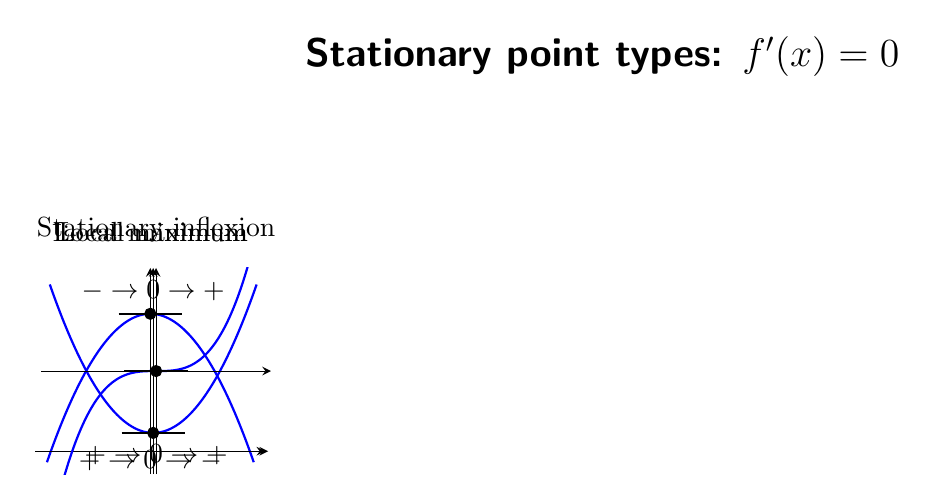
\begin{tikzpicture}

\node[font=\sffamily\Large\bfseries] at (7.2,5.3) {Stationary point types: $f'(x)=0$};

\begin{axis}[
    at={(0,0)},
    width=4.5cm,
    height=4.2cm,
    axis lines=middle,
    xmin=-2, xmax=2,
    ymin=-0.5, ymax=4,
    xtick=\empty,
    ytick=\empty,
    title={Local maximum},
    samples=100,
    domain=-1.8:1.8
]
\addplot[blue, thick] {-x^2+3};
\addplot[black, thick, domain=-0.55:0.55] {3};
\addplot[only marks, mark=*, black] coordinates {(0,3)};
\node at (axis cs:0,-0.2) {$+\to 0\to -$};
\end{axis}

\begin{axis}[
    at={(5,0)},
    width=4.5cm,
    height=4.2cm,
    axis lines=middle,
    xmin=-2, xmax=2,
    ymin=-0.5, ymax=4,
    xtick=\empty,
    ytick=\empty,
    title={Local minimum},
    samples=100,
    domain=-1.8:1.8
]
\addplot[blue, thick] {x^2+0.4};
\addplot[black, thick, domain=-0.55:0.55] {0.4};
\addplot[only marks, mark=*, black] coordinates {(0,0.4)};
\node at (axis cs:0,3.5) {$-\to 0\to +$};
\end{axis}

\begin{axis}[
    at={(10,0)},
    width=4.5cm,
    height=4.2cm,
    axis lines=middle,
    xmin=-2, xmax=2,
    ymin=-4, ymax=4,
    xtick=\empty,
    ytick=\empty,
    title={Stationary inflexion},
    samples=100,
    domain=-1.6:1.6
]
\addplot[blue, thick] {x^3};
\addplot[black, thick, domain=-0.55:0.55] {0};
\addplot[only marks, mark=*, black] coordinates {(0,0)};
\node at (axis cs:0,-3.25) {$+\to 0\to +$};
\end{axis}

\end{tikzpicture}
\end{document}
